\documentclass[%
  a4paper,%
  11pt,% <10pt, 9pt>
  %style=screen,
  %sender=bottom,
  blue,% <orange, green, violet>
  %rgb, <cmyk>
  %mono,
  hyperref	% tubs color for hyperref
  ]{tubsartcl}
\usepackage[utf8]{inputenc}
\usepackage{hyperref}

\setlength{\parindent}{0cm}
 
% Titelseiten-Elemente
\title{TuringBrain IDE \LARGE 1.0}
\subtitle{User Guide}
\author{\small Vanessa Baier, Nils Breyer, Phillipp Neumann,\\ Sven Schuster, David Wille}
\logo{
\includegraphics{ips}}
\titleabstract{TuringBrain IDE -- User Guide}
\titlepicture{title}
% Rückseiten-Elemente
\address{
  Advisor: Matthias Hagner\\\\
  Technische Universität Braunschweig\\
  Institut für Programmierung und Reaktive Systeme\\
  Mühlenpfordtstr. 23\\
  38106 Braunschweig}
\backpageinfo{
}

\begin{document}

\maketitle[image,logo=right]%[<plain/image/imagetext>,<logo=left/right>]

\tableofcontents
\newpage
\section{Introduction}

TuringBrain IDE allows you to develop and debug your own TuringMachines in an easy to use WYSIWYG (what you see is what you get) environment. It also enables you to program and run Brainfuck code.

\subsection{Features}

\begin{itemize}
  \item Edit Turing Machines by graphically editing the state graph
  \item Create Turing Machines with multiple tapes
  \item Write Brainfuck programs within the integrated code editor
  \item Simulate your machines and programs using the integrated simulation
  \item Simulate on special LEGO-Tape (hardware needed), graphically animated on the screen or on the console
  \item Pause simulation, Debug step-by-step
  \item Live-highlighting of the current state and edge during the simulation
  \item Save machines as .tm (an XML-Format) respective .bf
  \item Copy \& Paste (just for transitions on edges), Undo \& Redo
  \item Export to Latex, SVG, and PNG
  \item and many more features...
\end{itemize}

\section{Getting started}

\subsection{Installation}
\label{sec:installation}
If you don't want to use the LEGO tapes, you only have to download the executable .jar file from our repository.
To use the LEGO tapes you have to do following steps:
\begin{enumerate}
	\item Download Version 0.8.5beta of LeJos from http://sourceforge.net/projects/lejos/files/lejos-NXJ/
	\item Download JGraph from http://www.jgraph.com/jgraph.html
	\item Unpack the archive to a folder where you have execute privileges
	\item Download eclipse an install it
	\item Checkout our project as a new project with the wizzard of eclipse
	\item Choose in the wizzard Libraries and add the variable for jgraph-home and nxj-home
	\item Finish the project wizzard and compile the PC components with the external tool
	%%Wahrscheinlich noch nicht ganz fertig%%
\end{enumerate}


\newpage

\subsection{Welcome page}
\label{sec:welcome-page}
If the installation was correct and you have started the application the one or the other way you will see the welcome page like in figure \ref{pic:welcome_page}. Now you can open a turing machine, create a new one or open an example that is listed below. \\
You can also do the same with brainfuck applications.
\begin{figure}[!htb]
\begin{center}
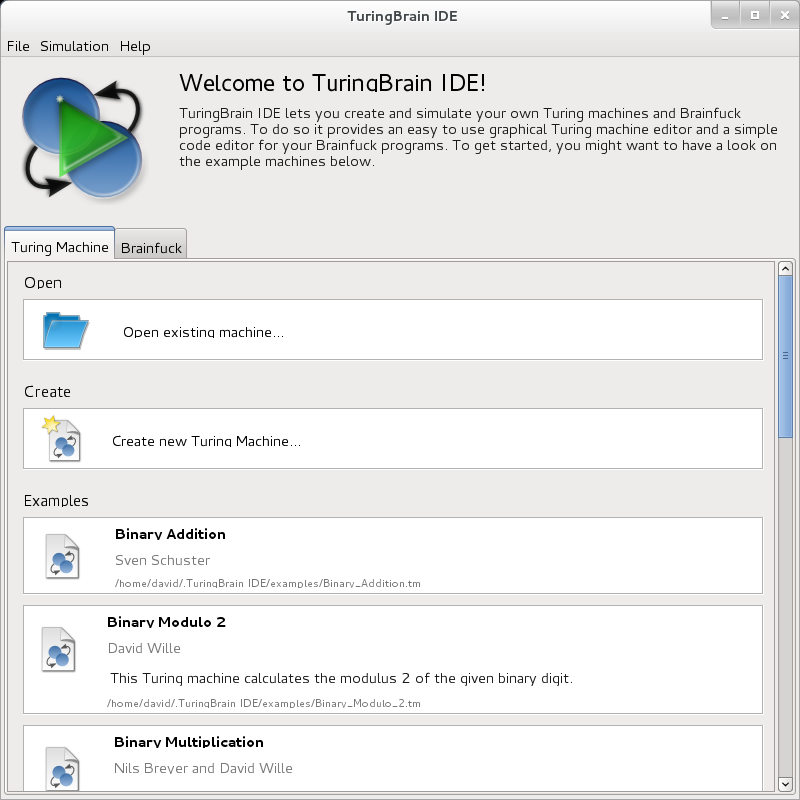
\includegraphics[scale=0.45]{graphics_gui/welcomescreen.png}
\end{center}
\caption{Welcome page}
\label{pic:welcome_page}
\end{figure}

\newpage

\section{Turing Machine editor}
If you open an example you will see a window like figure \ref{pic:turing_editor}, while creating a new machine leads to an empty window to work with. On the left side you see a toolbox (\ref{sec:toolbox}) and also there will be displayed panels to change the properties of the machine and all its components.
\begin{figure}[!htb]
\begin{center}
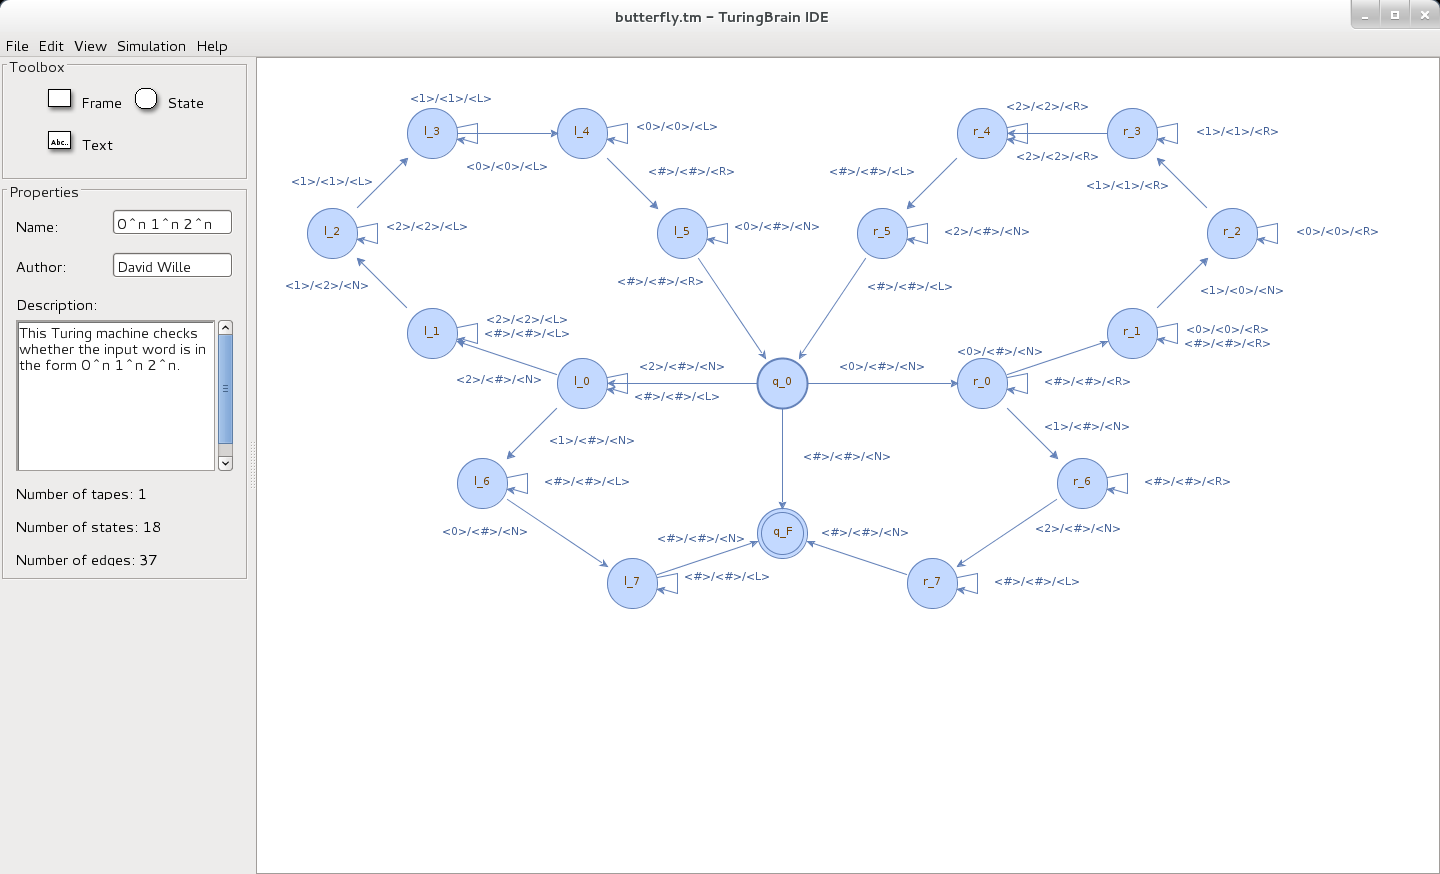
\includegraphics[scale=0.3]{graphics_gui/turing_editor.png}
\end{center}
\caption{Turing Machine editor}
\label{pic:turing_editor}
\end{figure}

\newpage

\subsection{Toolbox}
\label{sec:toolbox}
With the toolbox you can use drag an drop to add states, frames and textboxes to your machine. While states have a fixed size, frames and textboxes can be resized.
\begin{figure}[!htb]
\begin{center}
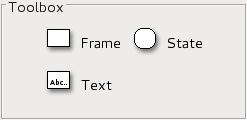
\includegraphics[scale=0.5]{graphics_gui/toolbox_turing.png}
\end{center}
\caption{Toolbox}
\label{pic:toolbox}
\end{figure}

\newpage

\subsection{Edit machine properties}
\label{sec:edit-mach-prop}
First of all you should edit the turing machine properties.
\begin{figure}[!htb]
\begin{center}
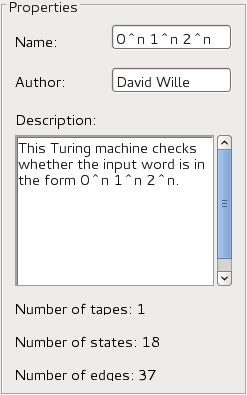
\includegraphics[scale=0.5]{graphics_gui/machine_properties.png}
\end{center}
\caption{Edit machine properties}
\label{pic:machine_properties}
\end{figure}

\newpage

\subsection{Adding and changing states}
\label{sec:add-edit-states}
If you have created or selected a state you can change the properties of the selected state. You can specify the label or whether it is a start and/or final state. The start state will be marked with a bold border and the final will be marked with a double circle.
\begin{figure}[!htb]
\begin{center}
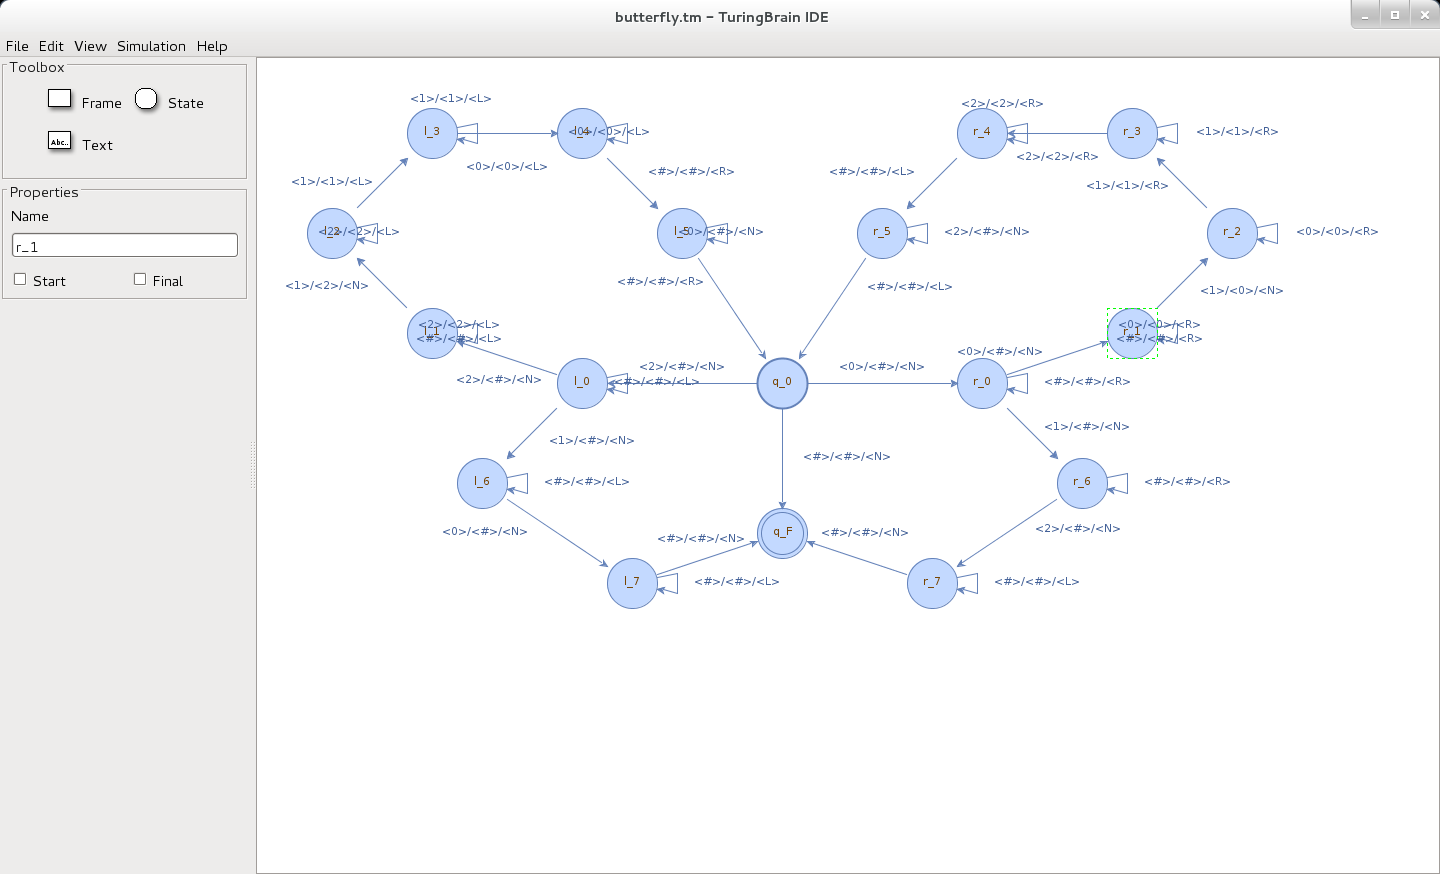
\includegraphics[scale=0.5]{graphics_gui/state_properties.png}
\end{center}
\caption{Adding and changing states}
\label{pic:state_properties}
\end{figure}

\newpage

\subsection{Adding and changing edges}
\label{sec:adding-chang-edges}
If you want to create an edge you have to move the mouse pointer to the center of a state, which will highlighted with a bold green square. Then you have to hold the left mouse button and drop the arrow on the state where the edge shall end. \\
If you have selected an edge you can add, remove or edit transitions. If you want to edit a transition you just have to double click on it.
\begin{figure}[!htb]
\begin{center}
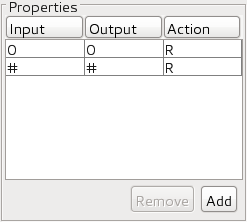
\includegraphics[scale=0.5]{graphics_gui/edge_properties.png}
\end{center}
\caption{Adding and changing edges}
\label{pic:edge_properties}
\end{figure}

\newpage

\subsection{Edit transitions}
\label{sec:edit-transitions}
If you double clicked on a transtion or added a new one, you can edit it. In general every character can be used, except for *, which is a wildcard. For LEGO tapes, allowed input and output characters are only \#, 0, 1, 2 and *. Allowed actions are L (left), R (right) an N (nothing).
\begin{figure}[!htb]
\begin{center}
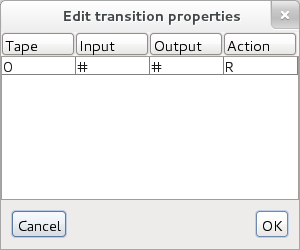
\includegraphics[scale=0.5]{graphics_gui/edit_transitions.png}
\end{center}
\caption{Edit transitions}
\label{pic:edit_transitions}
\end{figure}

\newpage

\subsection{Via points}
\label{sec:via-points}
When you select an edge you can add via points with Edit $>$ Add via point.

\subsection{Frames and textboxes}
\label{sec:frames-textboxes}
In the property toolbox of a textbox you can change the text of the box.
\begin{figure}[!htb]
\begin{center}
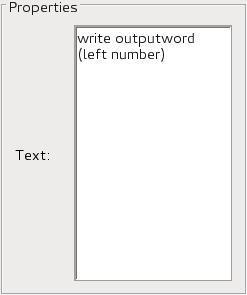
\includegraphics[scale=0.5]{graphics_gui/text_properties.png}
\end{center}
\caption{Textbox properties}
\label{pic:text_properties}
\end{figure}

\newpage

\subsection{Export}
\label{sec:export}
In the menu File->Export you can export the turing machine to Latex (.tex), Scalable Vector Graphic (.svg) or Portable Network Graphic (.png)
\newpage

\section{Brainfuck editor}
\label{sec:brainfuck-editor}
The Brainfuck editor  can be used to create applications using the esoteric programming language brainfuck. Our brainfuck interpreter differs a little from the original brainfuck implementation. Instead of an array of ASCII-symbols, we use a TuringMachine tape (Action) with only the symbols \#,0,1,2. Also the input and output strings are replaced by the tapes Input and Output.\\

The brainfuck language consists of only eight commands, each consisting of only one character:\\

\begin{tabular}{|c|l|}
\hline
\textbf{Command} & \textbf{Meaning} \\
\hline
$>$ & move to the next symbol on Action tape \\
\hline
$<$ & move to the previous symbol on Action tape \\
\hline
+ & increment symbol at current position on Action tape \\
\hline
- & decrement symbol at current position on Action tape \\
\hline
. & output symbol at current position on Action tape, symbol is written on Output tape \\
\hline
, & read next symbol from Input tape, writing it at current position on Action tape \\
\hline
[ & if current symbol is a \#, move to corresponding ] command, else execute following\\
\ & commands \\
\hline
] & if current symbol is not a \#, jump back to corresponding [ command \\
\hline
\end{tabular}

\bigskip
The commands are executed sequentially. Every other character within the code will be ignored.An example can be seen in figure \ref{pic:brainfuck_editor}.

\begin{figure}[!htb]
\begin{center}
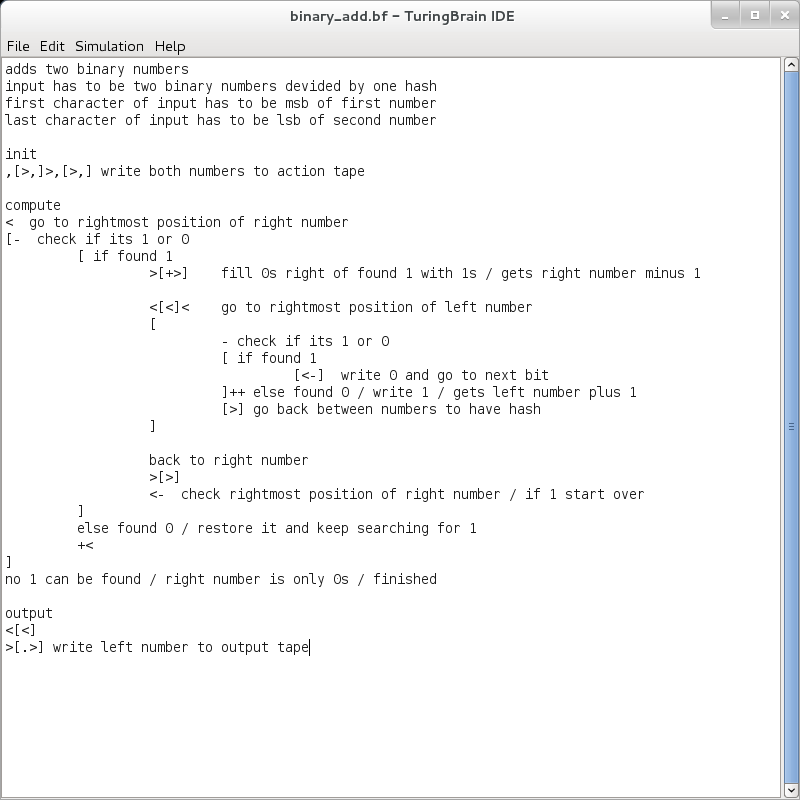
\includegraphics[scale=0.5]{graphics_gui/brainfuck_editor.png}
\end{center}
\caption{Brainfuck editor}
\label{pic:brainfuck_editor}
\end{figure}

\newpage

\section{Run window}

\begin{figure}[!htb]
\begin{center}
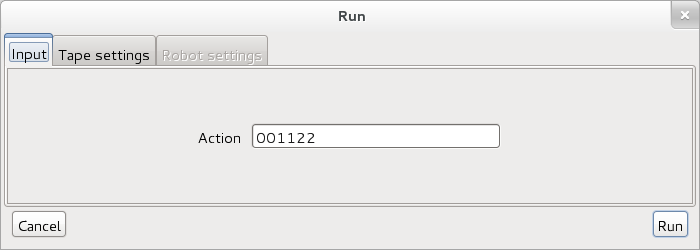
\includegraphics[scale=0.5]{graphics_gui/run_window_input.png}
\end{center}
\caption{Run window -- Input}
\label{pic:run_window_input}
\end{figure}

\newpage

\begin{figure}[!htb]
\begin{center}
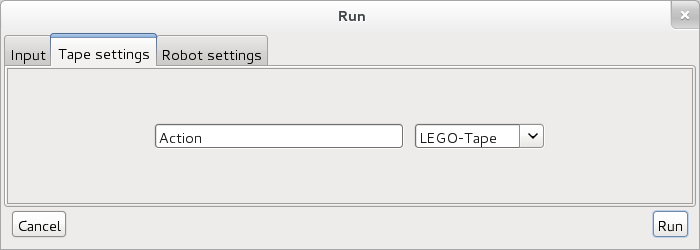
\includegraphics[scale=0.5]{graphics_gui/run_window_tape_settings.png}
\end{center}
\caption{Run window -- Tape settings}
\label{pic:run_window_tape_settings}
\end{figure}

\newpage

\begin{figure}[!htb]
\begin{center}
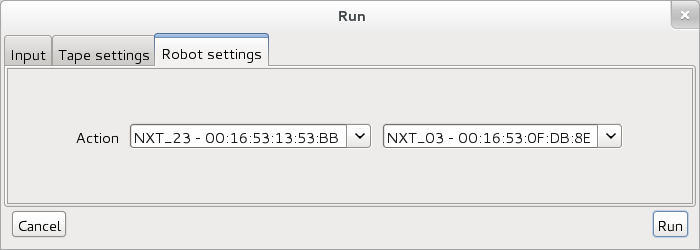
\includegraphics[scale=0.5]{graphics_gui/run_window_robot_settings.png}
\end{center}
\caption{Run window -- Robot settings}
\label{pic:run_window_robot_settings}
\end{figure}

\newpage

\section{Simulation}

\subsection{Organize robots}

\begin{figure}[!htb]
\begin{center}
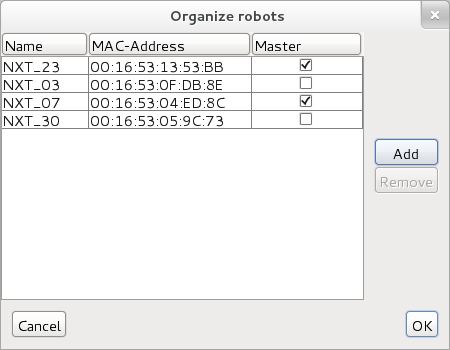
\includegraphics[scale=0.45]{graphics_gui/organize_robots.png}
\end{center}
\caption{Organize robots}
\label{pic:organize_robots}
\end{figure}

\newpage

\subsection{Presimulation window}

\begin{figure}[!htb]
\begin{center}
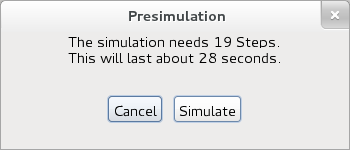
\includegraphics[scale=0.4]{graphics_gui/presimulation.png}
\end{center}
\caption{Presimulation window}
\label{pic:presimulation}
\end{figure}

\begin{figure}[!htb]
\begin{center}
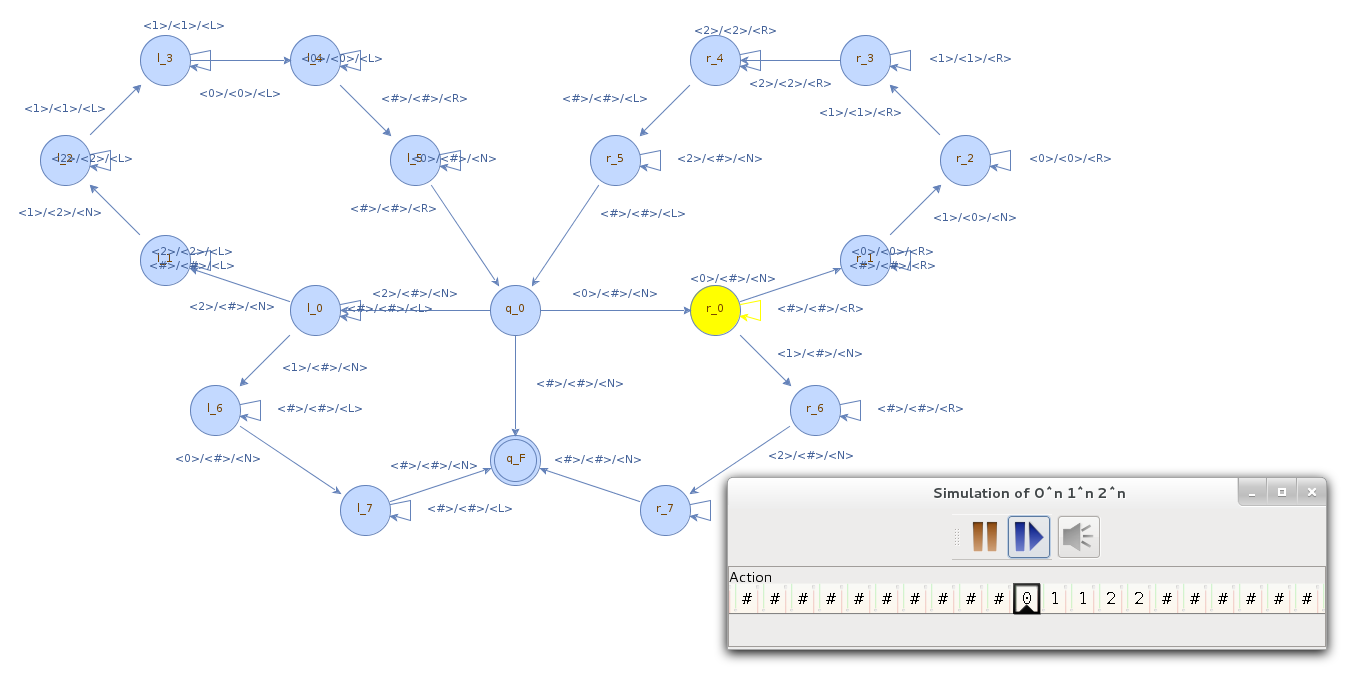
\includegraphics[scale=0.35]{graphics_gui/simulation_window.png}
\end{center}
\caption{Simulation window}
\label{pic:simulation_window}
\end{figure}

\newpage

\section{Hardware -- LEGO\textregistered\, tape}

This section describes the position of the components used in the machine. The following subsections and pictures are meant to extend the building instructions file created with the LEGO\textregistered\, Digital Designer.

\subsection{The machine's motor section}

Figure \ref{pic:topview} shows a view of the machine's motor section to get a brief overview of it's position and the number 1 -- 4 represent the following pictures.

\begin{figure}[!htb]
\begin{center}
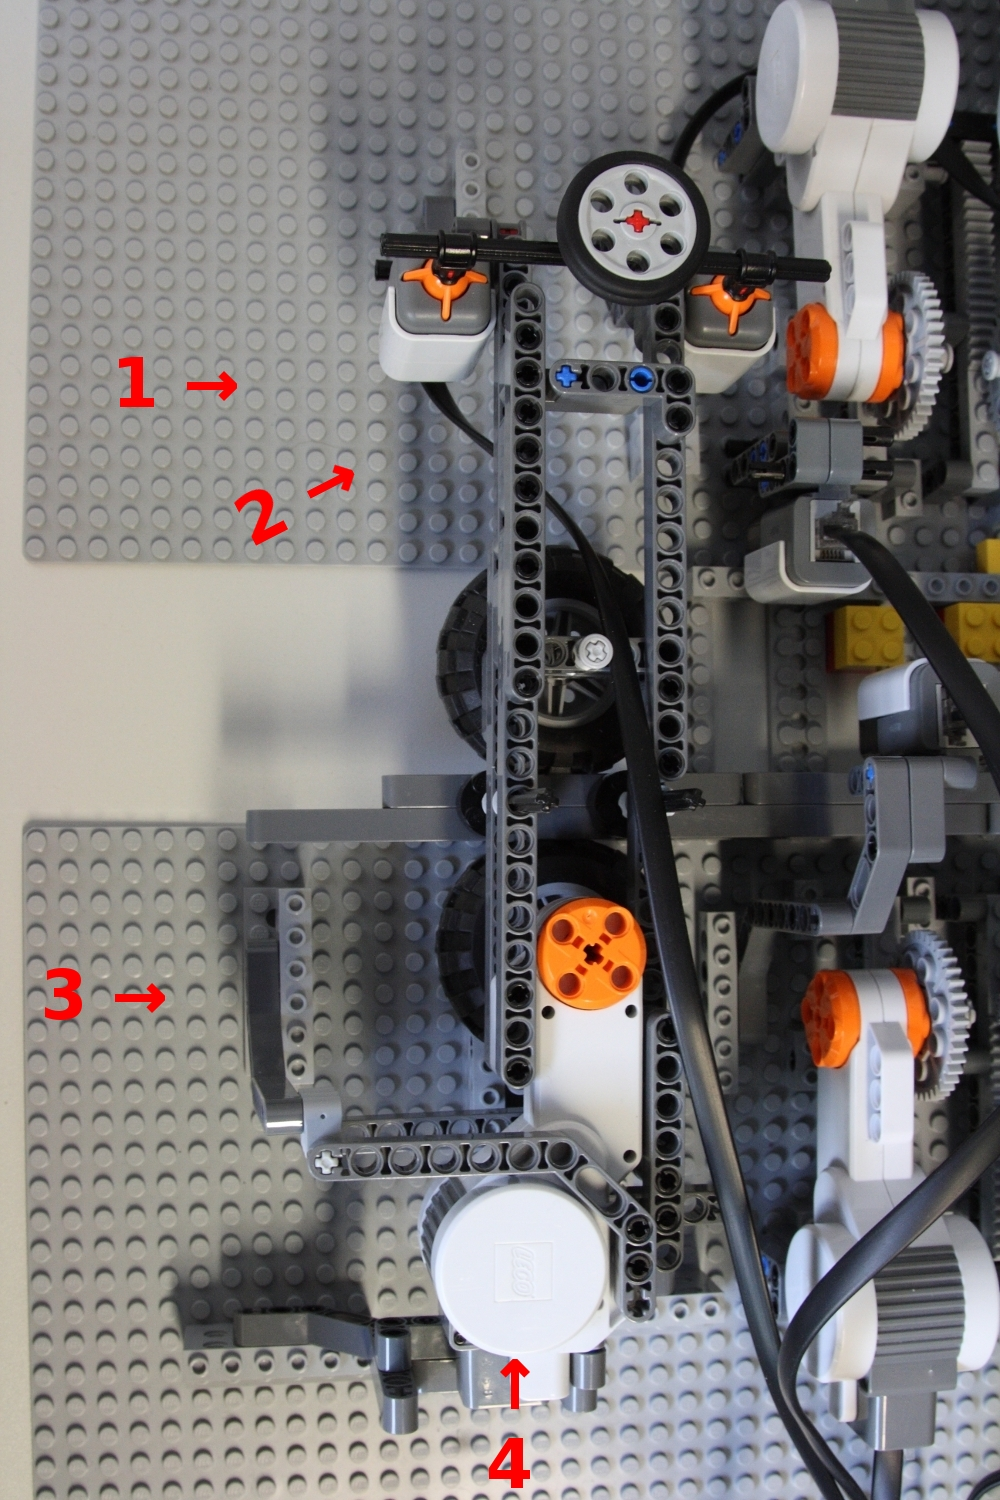
\includegraphics[scale=0.28]{graphics_lego/topview.jpg}
\end{center}
\caption{Overview of the motor section}
\label{pic:topview}
\end{figure}

\newpage

Figure \ref{pic:position1} shows how the upper left pier has to be placed in relation to the left edge of the upper plate.

\begin{figure}[!htb]
\begin{center}
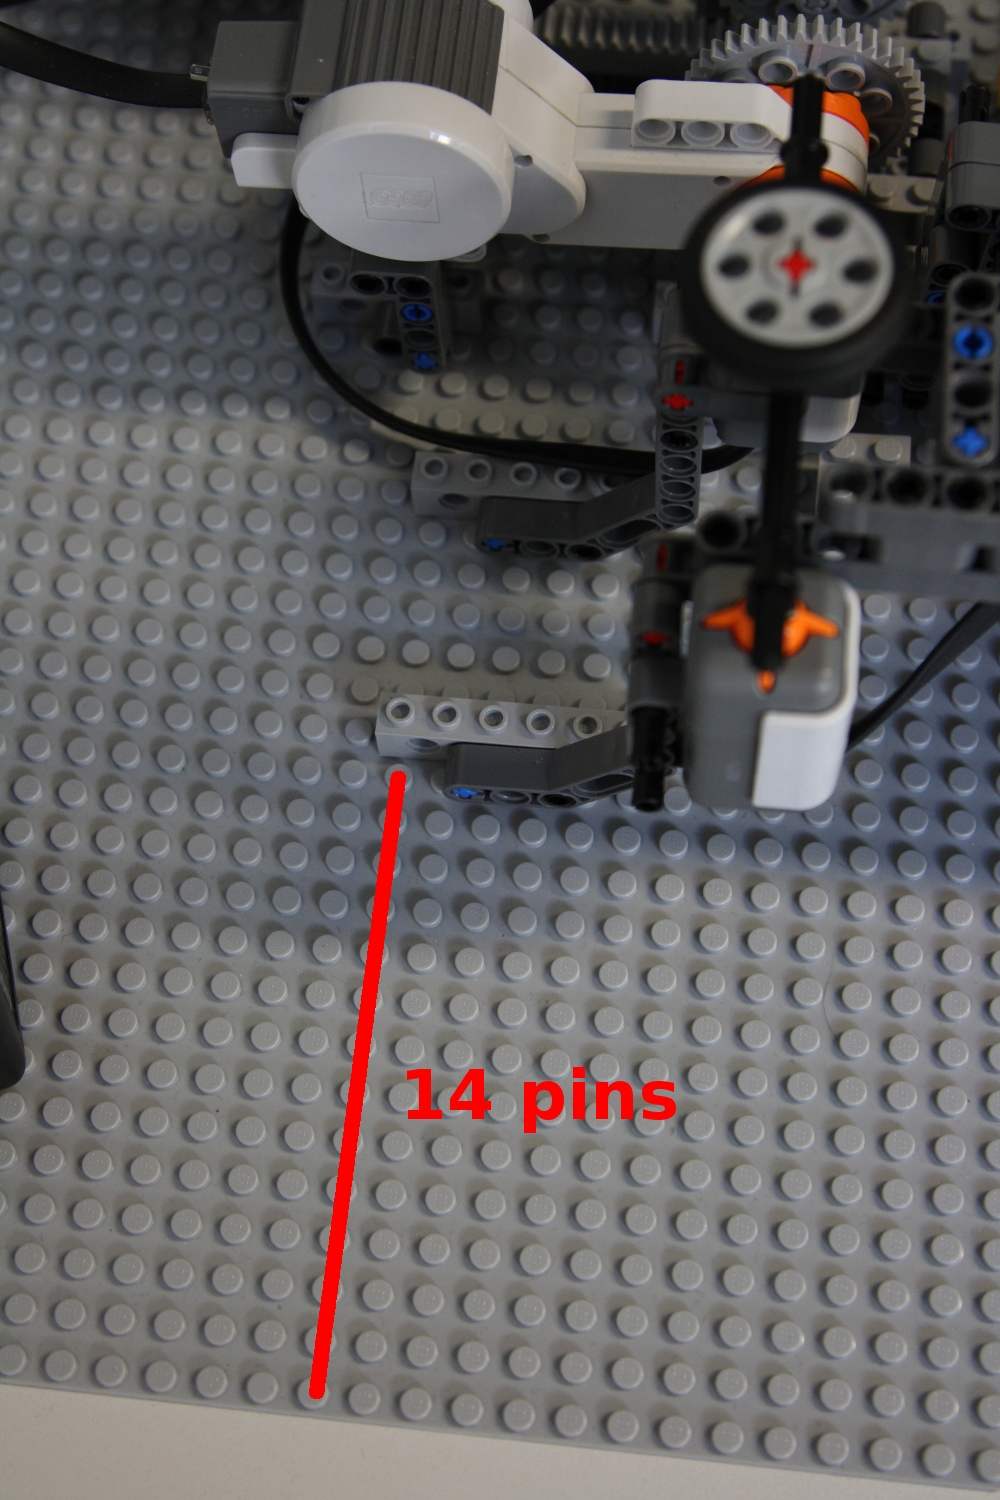
\includegraphics[scale=0.35]{graphics_lego/position1.jpg}
\end{center}
\caption{Image taken from position 1}
\label{pic:position1}
\end{figure}

\newpage

Figure \ref{pic:position2} shows how the upper left and right pier have to be placed in relation to the bottom edge of the upper plate.

\begin{figure}[!htb]
\begin{center}
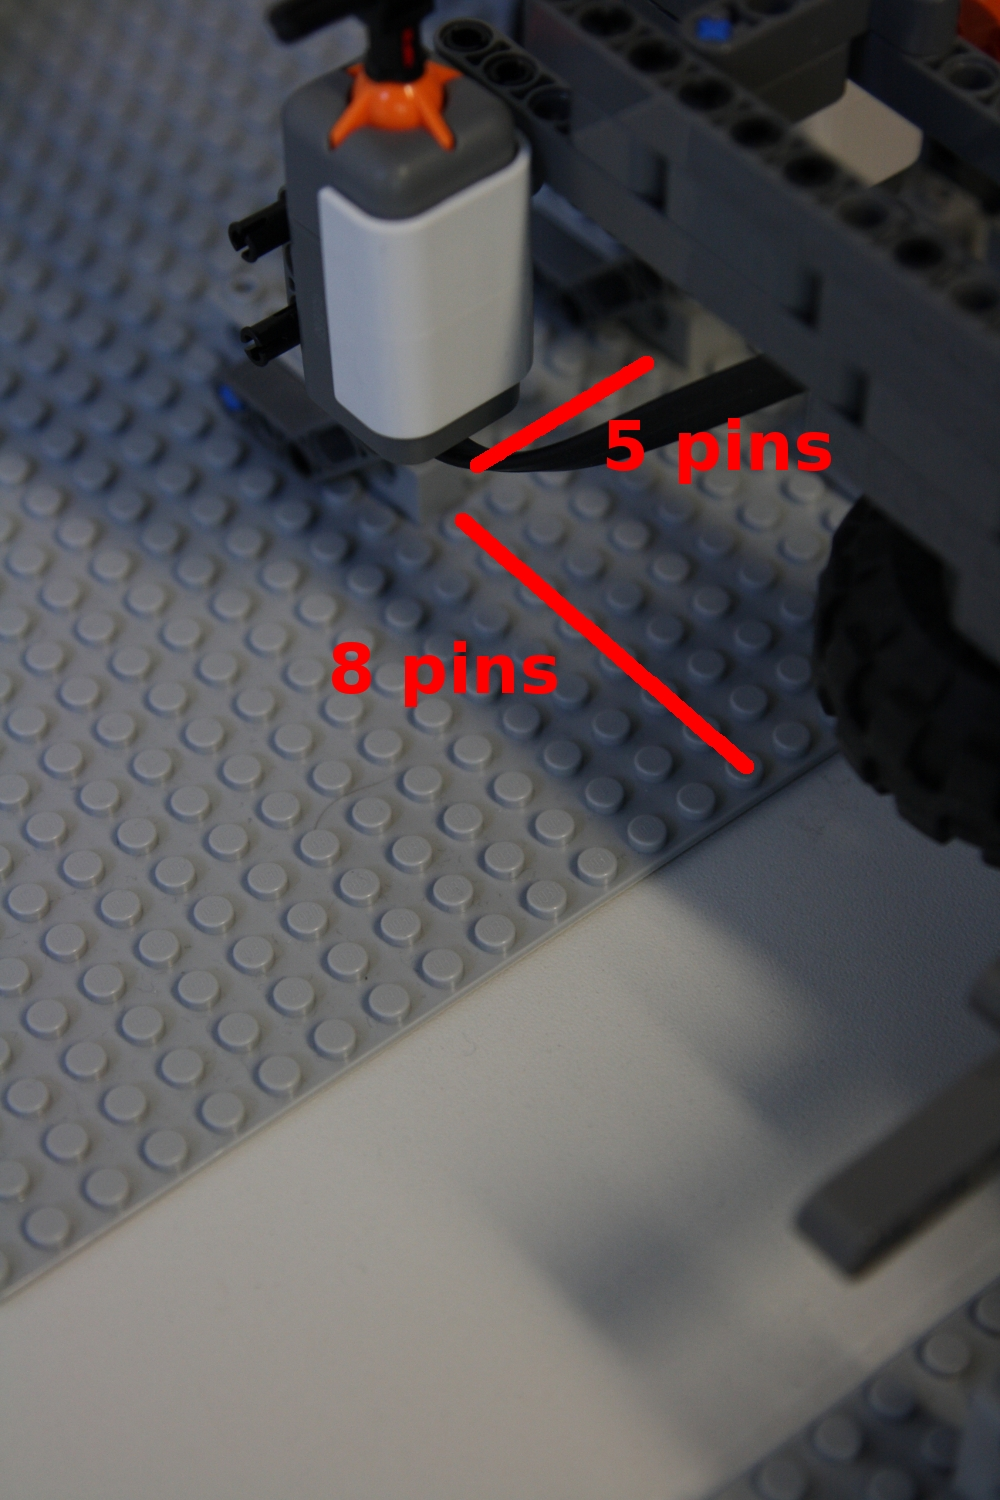
\includegraphics[scale=0.35]{graphics_lego/position2.jpg}
\end{center}
\caption{Image taken from position 2}
\label{pic:position2}
\end{figure}

\newpage

Figure \ref{pic:position3} shows how the lower left piers have to be placed in relation to the top and left edge of the lower plate.

\begin{figure}[!htb]
\begin{center}
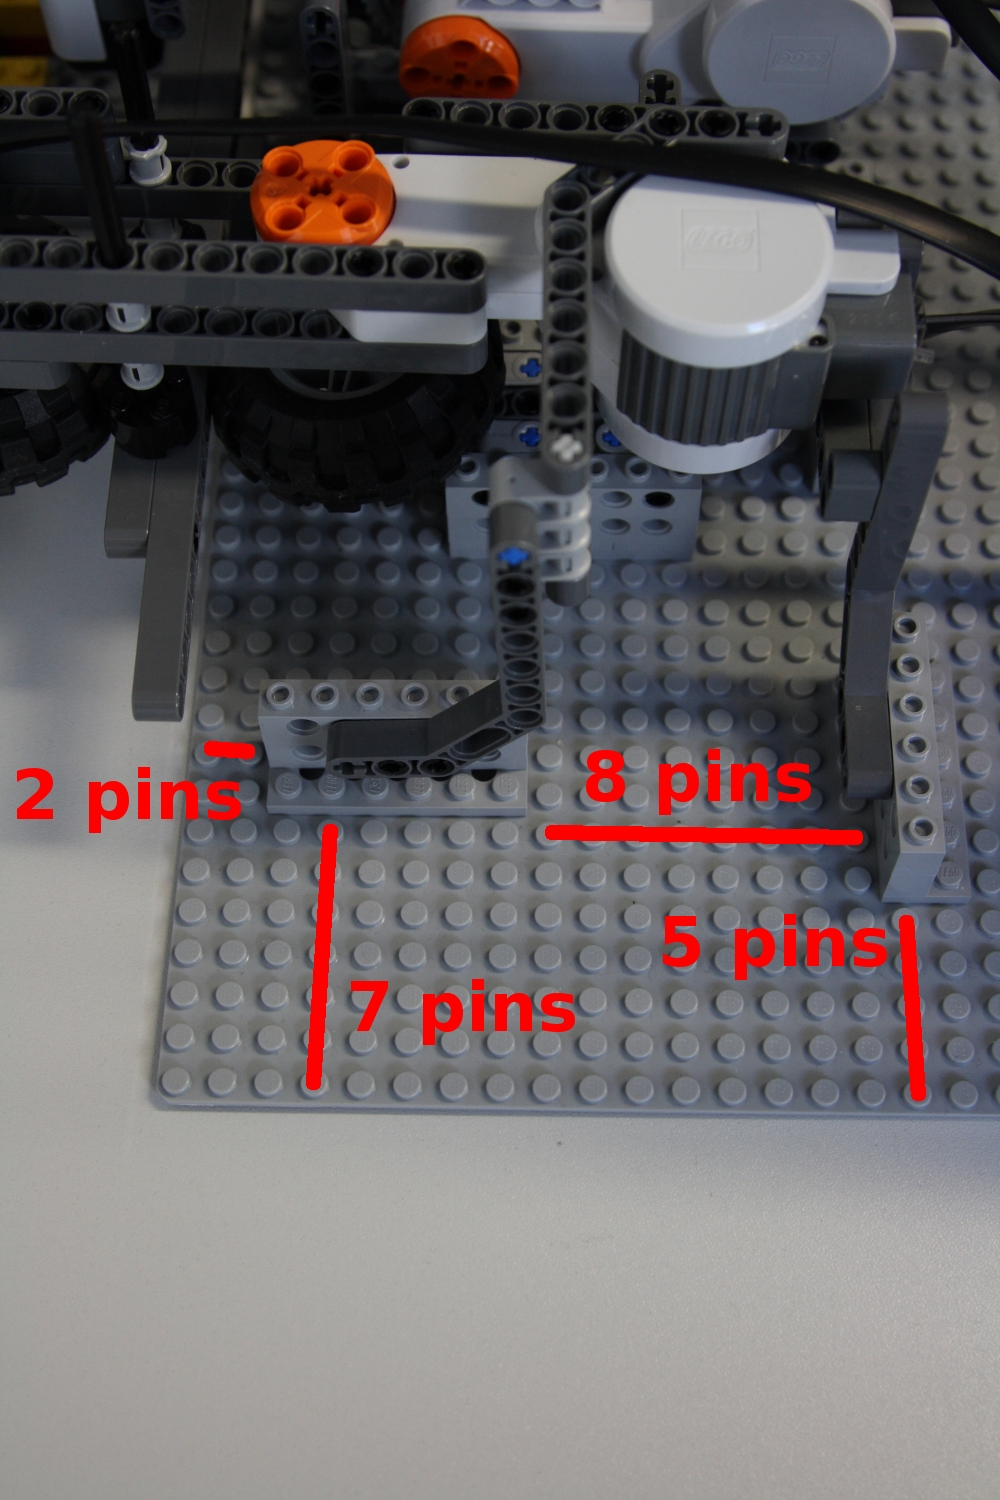
\includegraphics[scale=0.35]{graphics_lego/position3.jpg}
\end{center}
\caption{Image taken from position 3}
\label{pic:position3}
\end{figure}

\newpage

Figure \ref{pic:position4} shows how the lower right pier has to be placed in relation to the left pier and the support for the motor wheel.

\begin{figure}[!htb]
\begin{center}
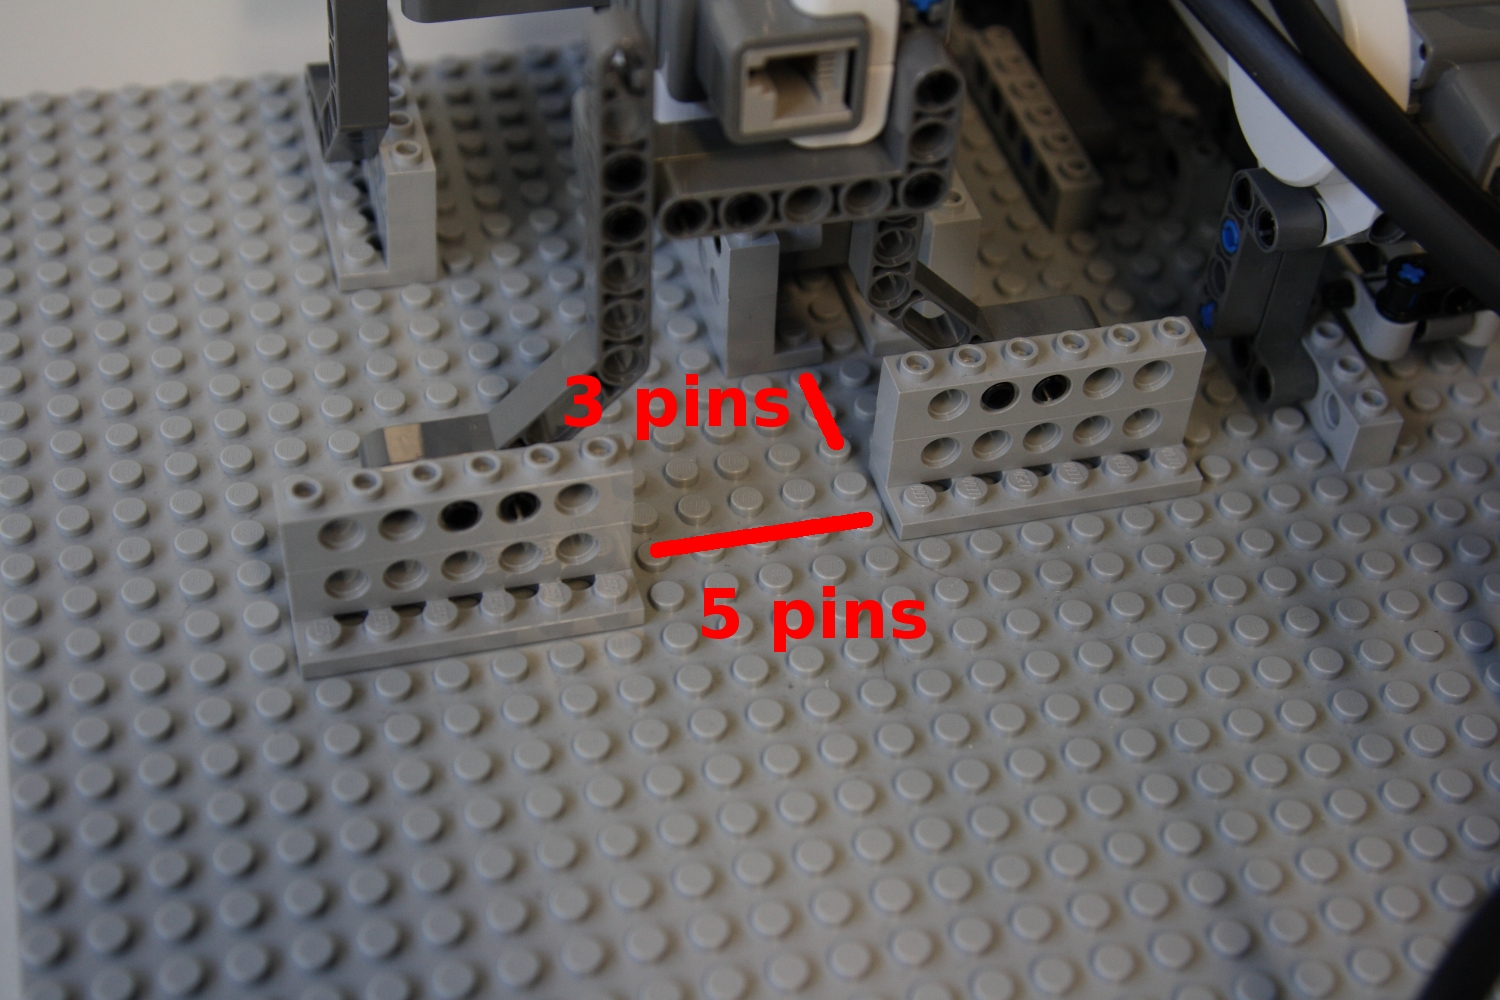
\includegraphics[scale=0.3]{graphics_lego/position4.jpg}
\end{center}
\caption{Image taken from position 4}
\label{pic:position4}
\end{figure}

\newpage

\subsection{The supporting bridge at the end of the tape}

Figure \ref{pic:bridge2} shows how the upper piers of the supporting bridge have to be placed in relation to the lower and right edge of the upper plate.

\begin{figure}[!htb]
\begin{center}
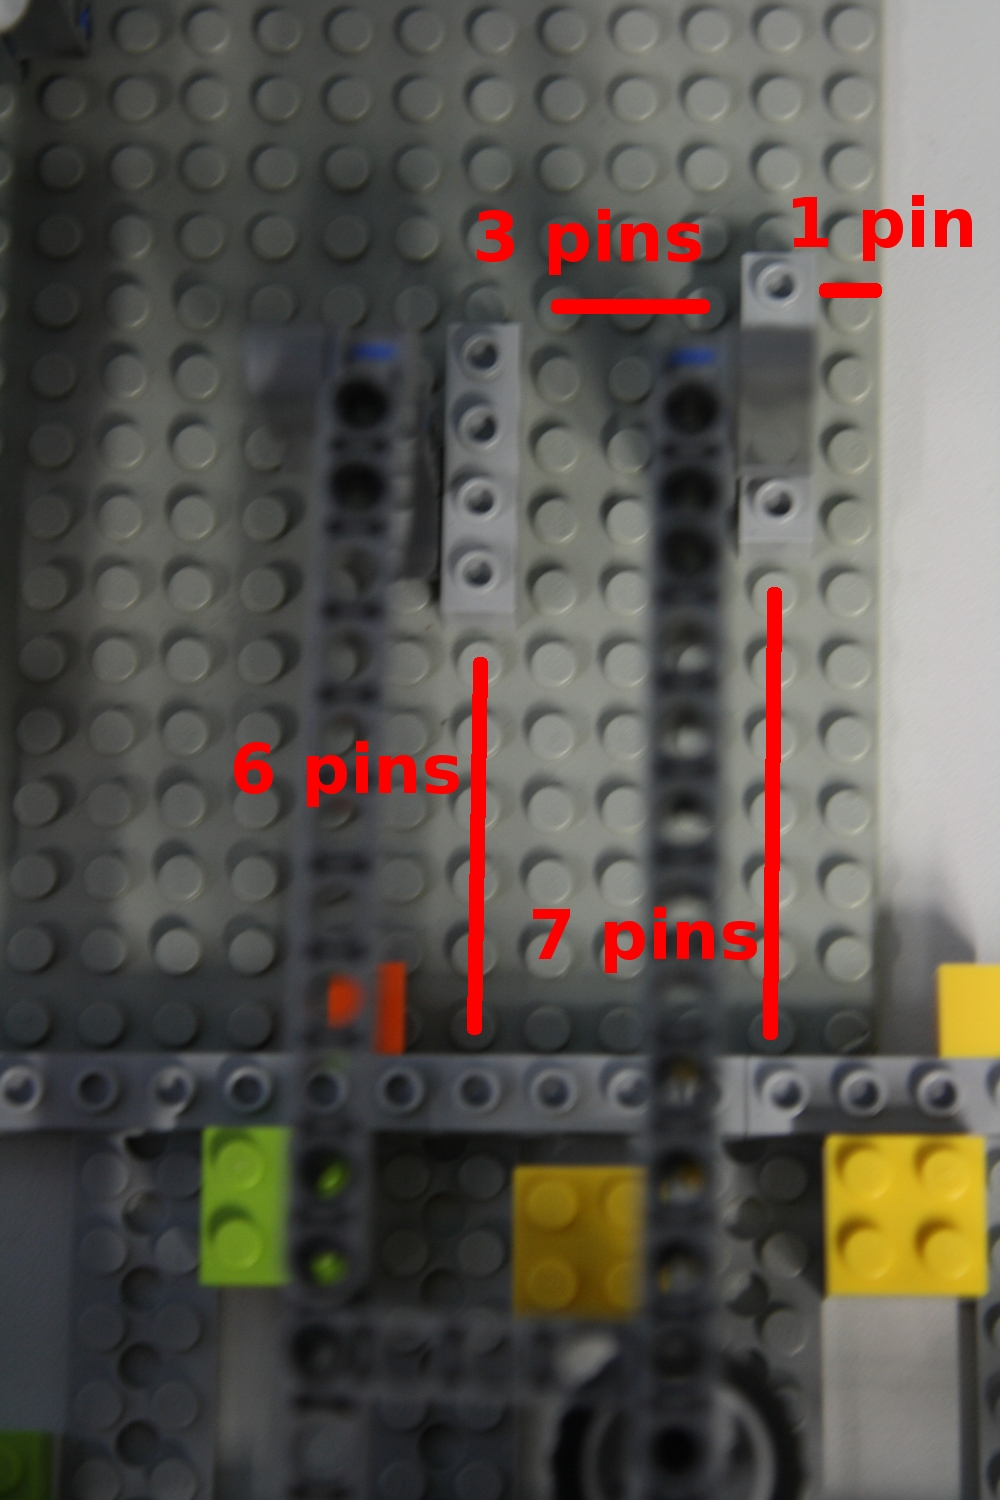
\includegraphics[scale=0.35]{graphics_lego/bridge2.jpg}
\end{center}
\caption{Position of the bridge}
\label{pic:bridge2}
\end{figure}

\newpage

Figure \ref{pic:bridge1} shows how the lower piers of the supporting bridge have to be placed in relation to the upper and right edge of the lower plate.

\begin{figure}[!htb]
\begin{center}
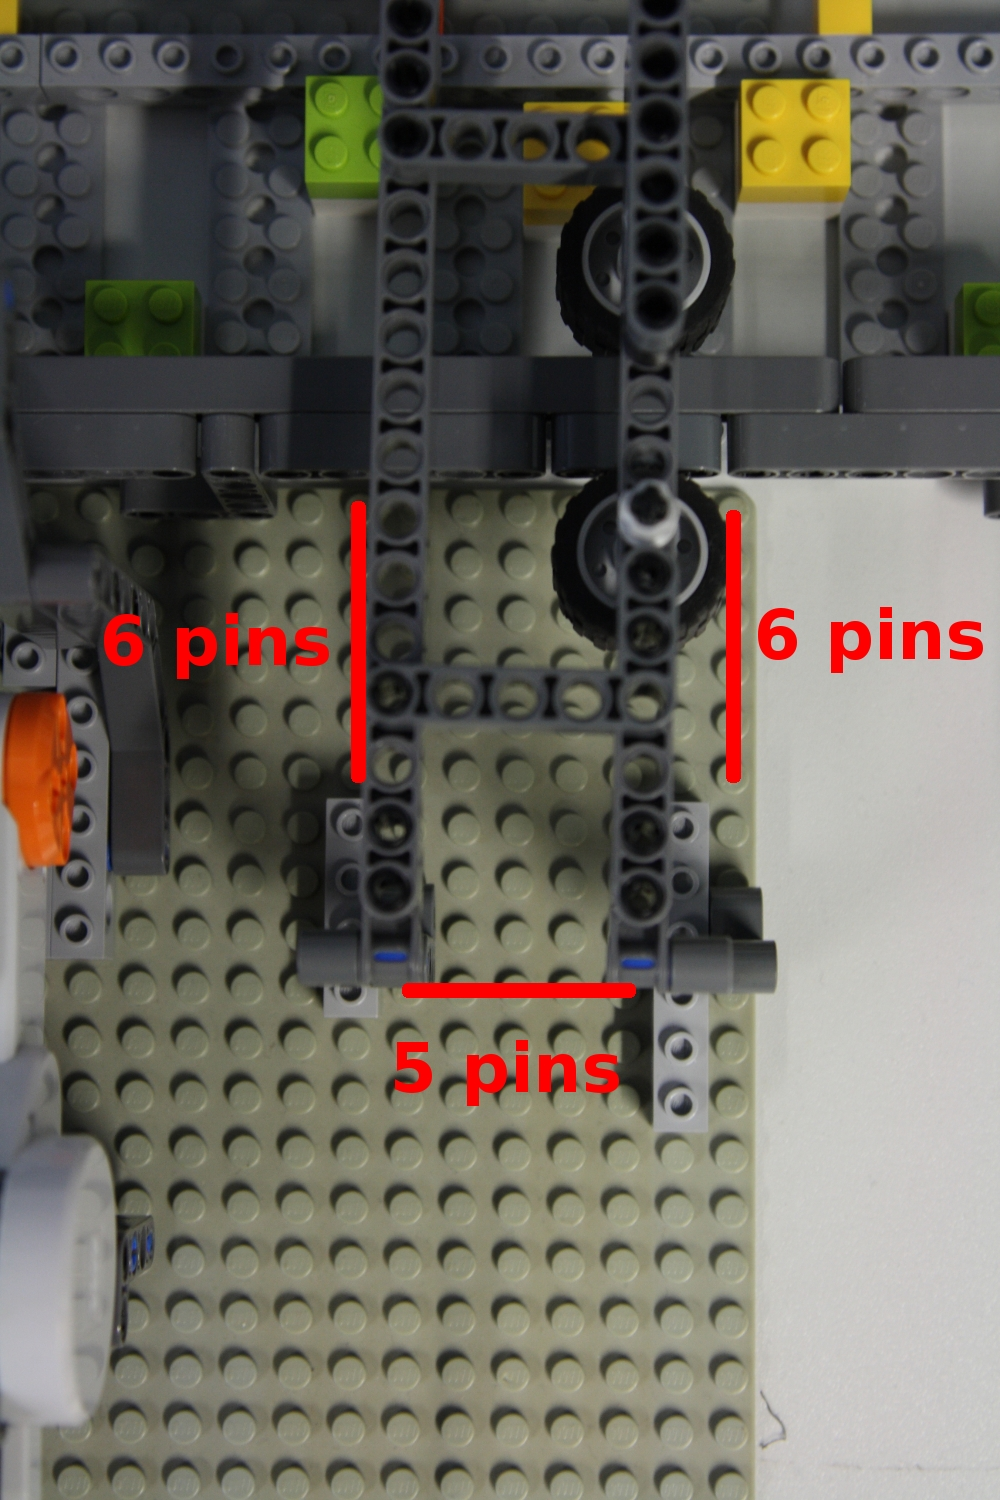
\includegraphics[scale=0.35]{graphics_lego/bridge1.jpg}
\end{center}
\caption{Position of the bridge}
\label{pic:bridge1}
\end{figure}

\newpage

\subsection{The sensors}

Figure \ref{pic:sensors} shows how the sensors have to be placed to work properly. As you can see the sensor it the rectangle 1 has to be above one of the position bits every time the sensors in rectangle 2 are above two bits at one of the positions.

\begin{figure}[!htb]
\begin{center}
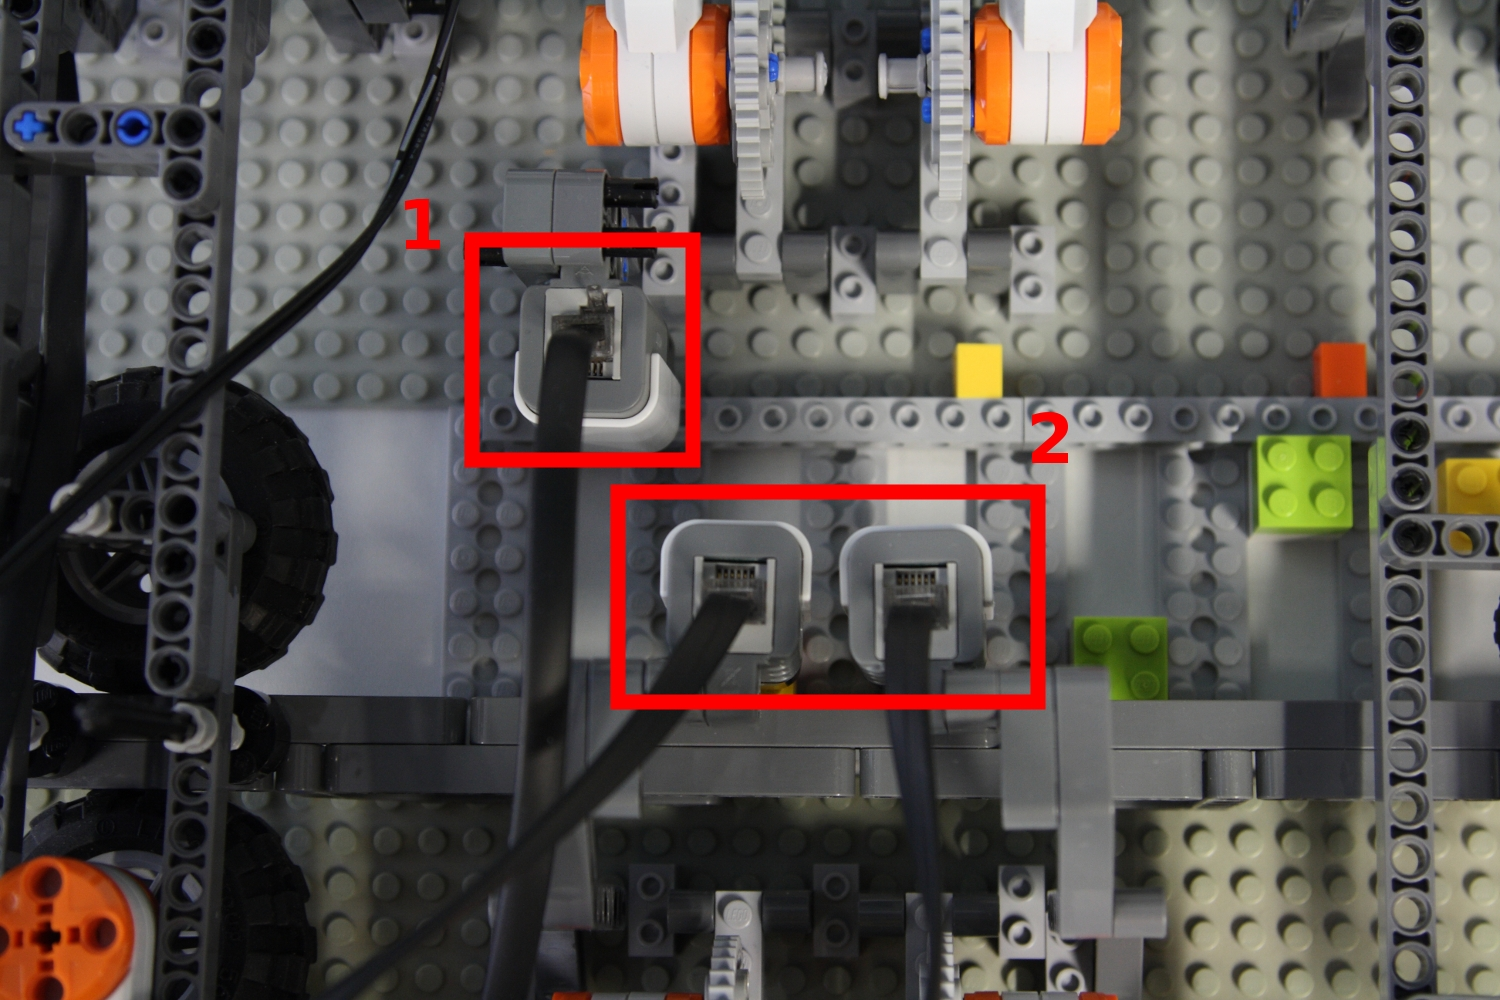
\includegraphics[scale=0.3]{graphics_lego/sensors.jpg}
\end{center}
\caption{Position of the sensors}
\label{pic:sensors}
\end{figure}

\newpage

\subsection{The tape}

The Marker in Figure \ref{pic:tape} shows how the bricks have to be placed so the sensors recognize them and can distinguish the different positions of the tape. It is also very important that the piers used for the upper bar of the tape are not interfering with the pushers shown in Figure \ref{pic:topview_pushers} and Figure \ref{pic:pusher}. So the pier you can see in the background of Figure \ref{pic:tape} is placed perfectly because it is not preventing the pushers from moving the bits.

\begin{figure}[!htb]
\begin{center}
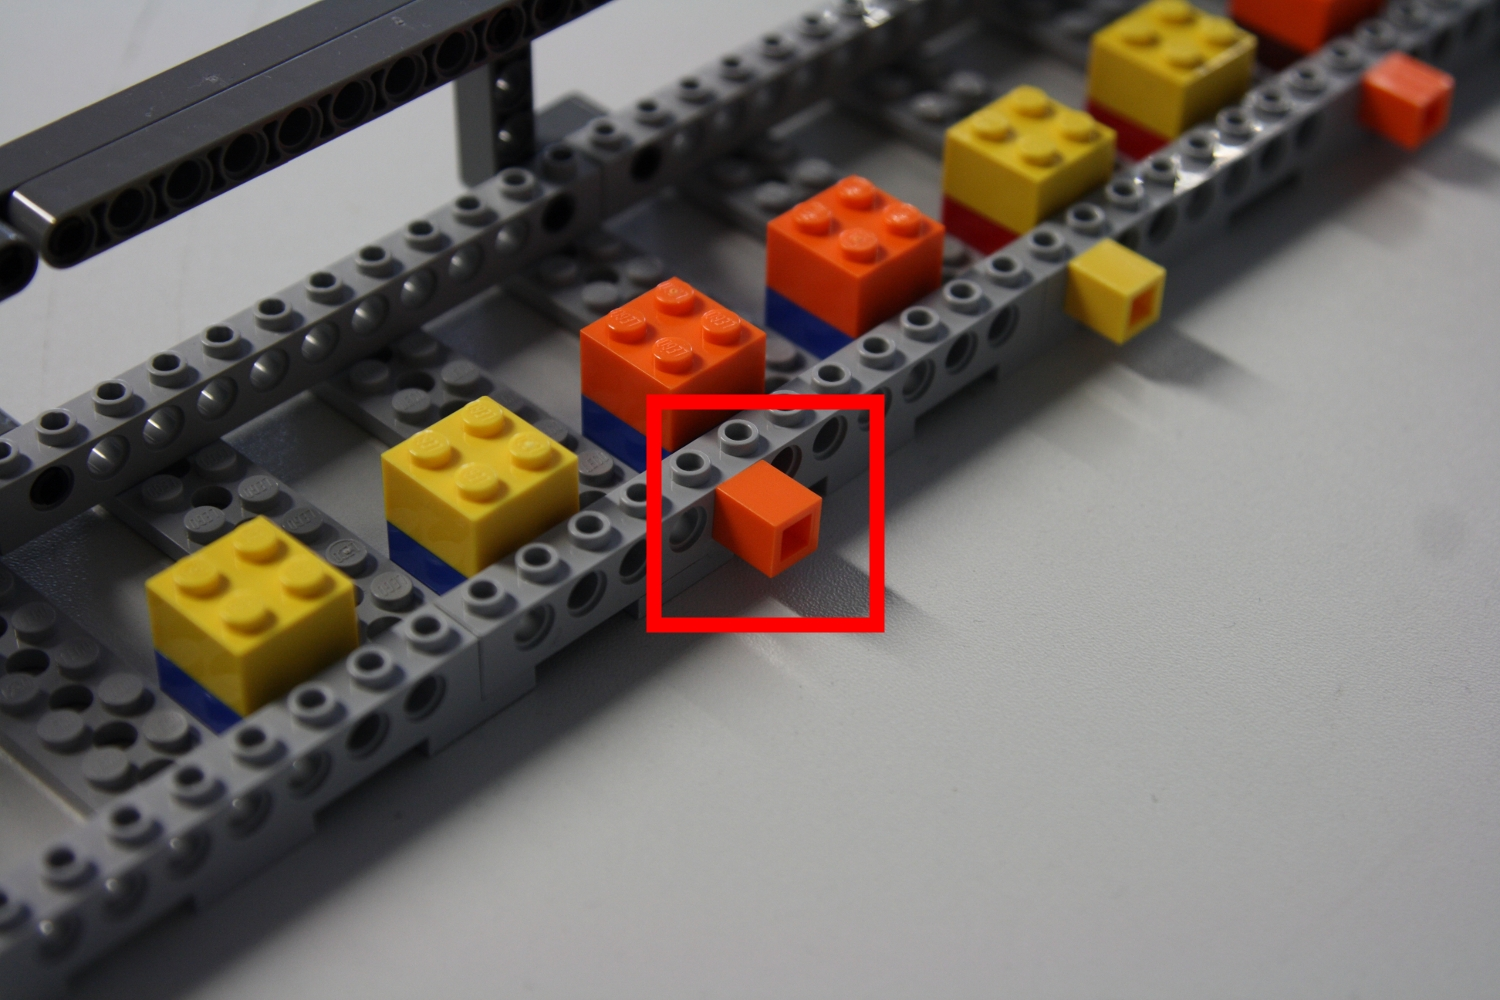
\includegraphics[scale=0.3]{graphics_lego/tape.jpg}
\end{center}
\caption{The tape}
\label{pic:tape}
\end{figure}

\newpage

Figure \ref{pic:supporting_pier} shows how the supporting piers have to be placed so they do not interfere with the pushers. It also shows how the sensors in the rectangle 2 in figure \ref{pic:sensors} have to be placed so they are above the bits every time the sensor in rectangle 1 is above a position bit.

\begin{figure}[!htb]
\begin{center}
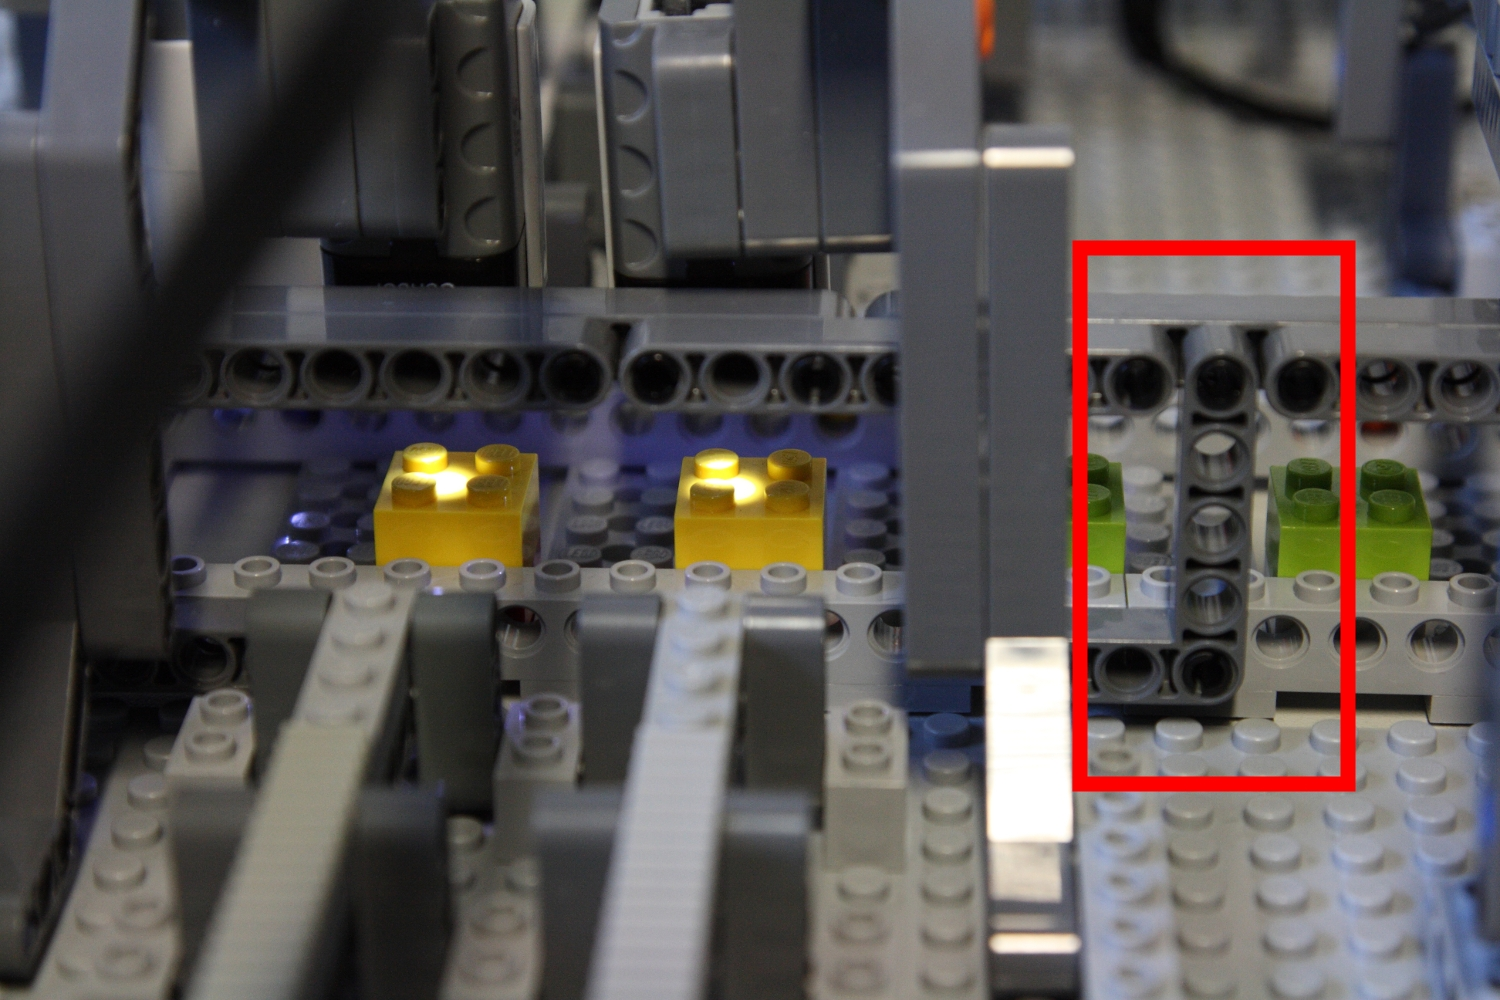
\includegraphics[scale=0.3]{graphics_lego/supporting_pier.jpg}
\end{center}
\caption{One of the supporting piers}
\label{pic:supporting_pier}
\end{figure}

\newpage

\subsection{The pushers}

Figure \ref{pic:pusher} shows how the pushers have to be placed on the guard rail so they can be pushed properly by the gear wheels. It also shows how the gear wheel has to be placed on the pusher so it pushes properly.

\begin{figure}[!htb]
\begin{center}
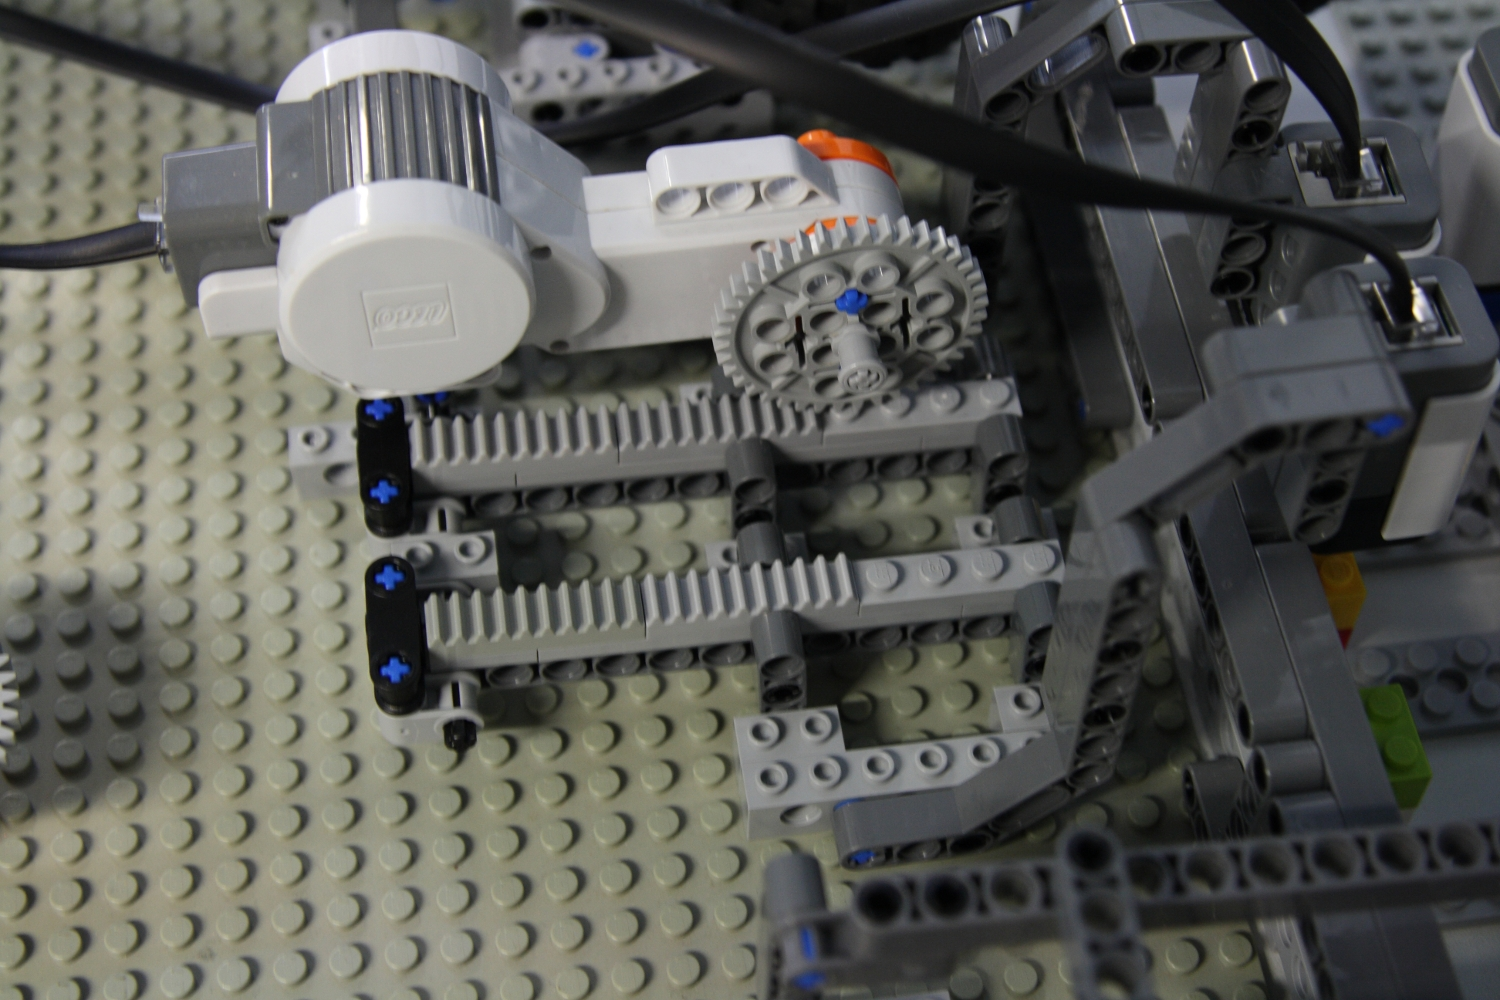
\includegraphics[scale=0.3]{graphics_lego/pusher.jpg}
\end{center}
\caption{Pusher}
\label{pic:pusher}
\end{figure}

\newpage

Figure \ref{pic:topview_pushers} shows how the pushers are pushing the bits and how to place the supporting piers (rectangle) for the tape's upper bar so they do not interfere with the pushers.

\begin{figure}[!htb]
\begin{center}
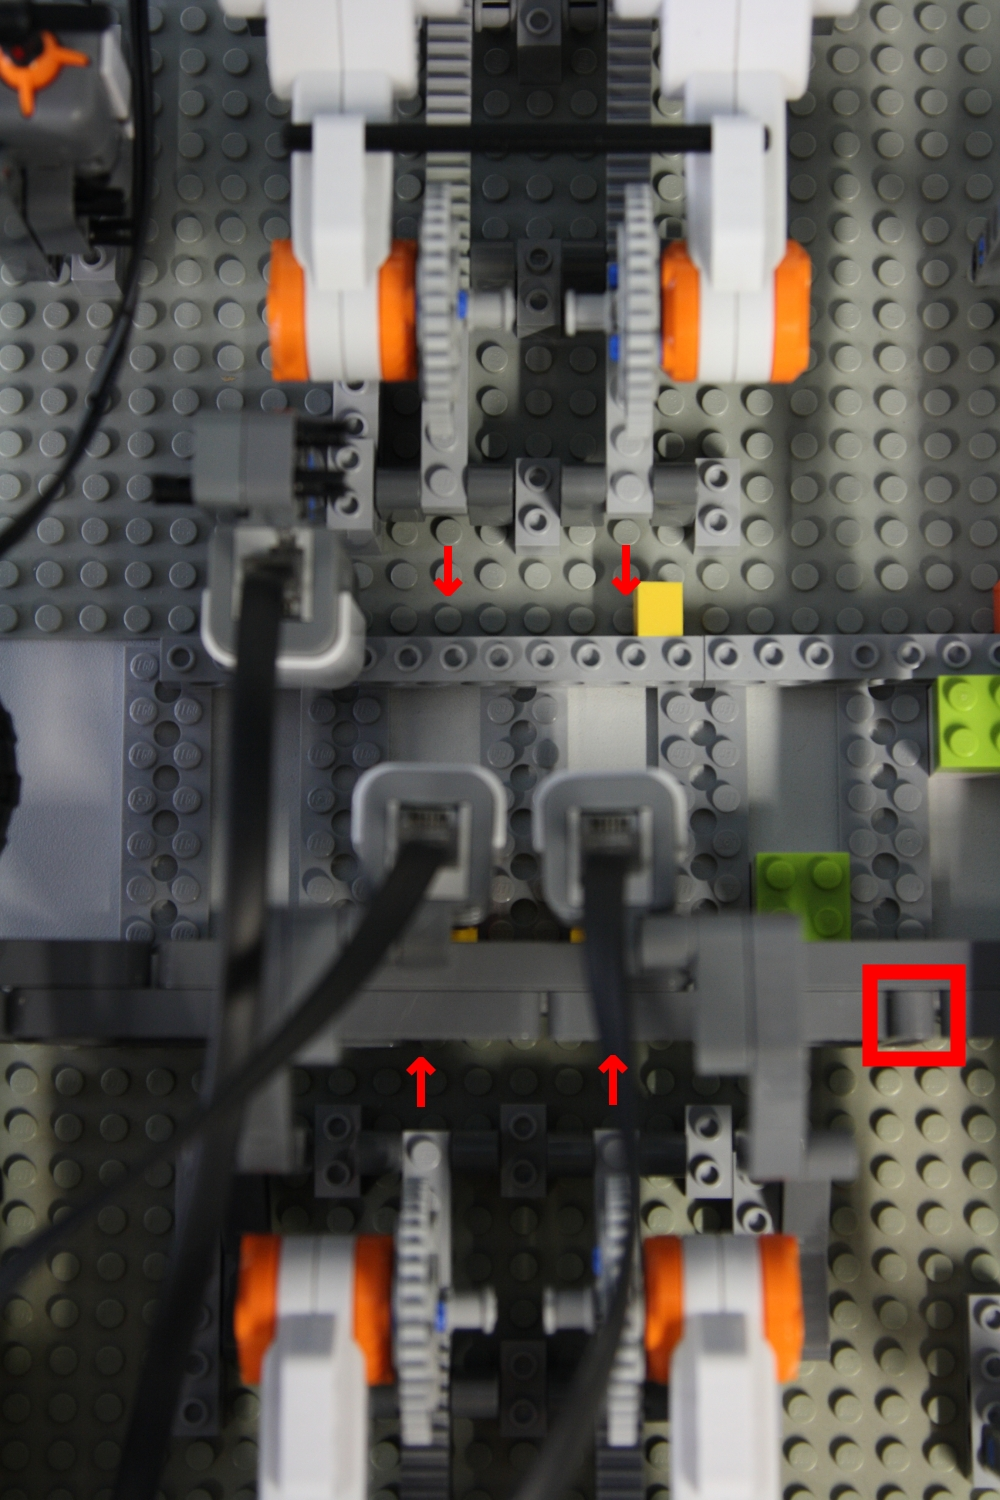
\includegraphics[scale=0.35]{graphics_lego/topview_pushers.jpg}
\end{center}
\caption{Position of the pushers}
\label{pic:topview_pushers}
\end{figure}


\section{Code -- LEGO\textregistered\, tape}

\subsection{Master NXT module}

\subsubsection{Image}

\subsubsection{MainMaster}

\subsection{Slave NXT module}

\subsubsection{MainSlave}

\subsubsection{TetrisSound}


\subsection{Common NXT classes}

\subsubsection{Calibrate}

\subsubsection{Common}

\subsubsection{Tape}

\subsubsection{Timer}

\subsubsection{SensorTest}


\section{Code -- GUI}


\subsection{Package gui}

\subsubsection{AboutDialog}

\subsubsection{AppData}

\subsubsection{CustomTable}

\subsubsection{Editor}

\subsubsection{ErrorDialog}

\subsubsection{MachineEditor}

\subsubsection{OrganizeRobots}

\subsubsection{PresimulationDialogue}

\subsubsection{RunWindow}

\subsubsection{SimulationWindow}

\subsubsection{WelcomeScreen}

\subsubsection{WelcomeScreenGroup}

\subsubsection{WelcomeScreenLine}

\subsection{Package gui.brainfuck}

\subsubsection{BrainfuckEditor}


\subsection{Package gui.turing}

\subsubsection{NewTMDialogue}

\subsubsection{Palette}

\subsubsection{PropertiesEdge}

\subsubsection{PropertiesEdgeEdit}

\subsubsection{PropertiesState}

\subsubsection{PropertiesTextbox}

\subsubsection{PropertiesTuringMachine}

\subsubsection{ToolBox}

\subsubsection{TuringMachineEditor}


\subsection{Package machine}

\subsubsection{ExtensionFileFilter}

\subsubsection{Machine}

\subsubsection{Simulation}


\subsubsection{Package machine.brainfuck}

\subsubsection{BrainfuckMachine}

\subsubsection{BrainfuckSimulation}


\subsection{Package machine.turing}

\subsubsection{Edge}

\subsubsection{Frame}

\subsubsection{InOut}

\subsubsection{Point}

\subsubsection{State}

\subsubsection{Textbox}

\subsubsection{Transition}

\subsubsection{TuringMachine}

\subsubsection{TuringSimulation}


\subsection{Package tape}

\subsubsection{ConsoleTape}

\subsubsection{DisplayableTape}

\subsubsection{GraphicTape}

\subsubsection{GraphicTapePanel}

\subsubsection{LEGOTape}

\subsubsection{MasterRobot}

\subsubsection{Robot}

\subsubsection{SlaveRobot}


\subsubsection{Tape}

\subsubsection{TapeException}


\makebackpage[trisec]%[<plain/info/addressinfo>]

\end{document}
